\chapter{Resultat}

Som forventet, afsender klienten en anmodning om hhv uptime og load i figur \ref{fig:uptimeclient} og figur \ref{fig:loadclient}, der modtages af serveren, som herpå indlæser den efterspurgte data og sender tilbage til klienten, som det fremgår af figur \ref{fig:uptimeserver} og figur \ref{fig:loadserver}, der midlertidigt bare står og lytter efter svar.

Når klienten modtager svaret, udskriver den det til terminalen og afslutter. 

\begin{figure}[h!]
	\centering
	\fbox{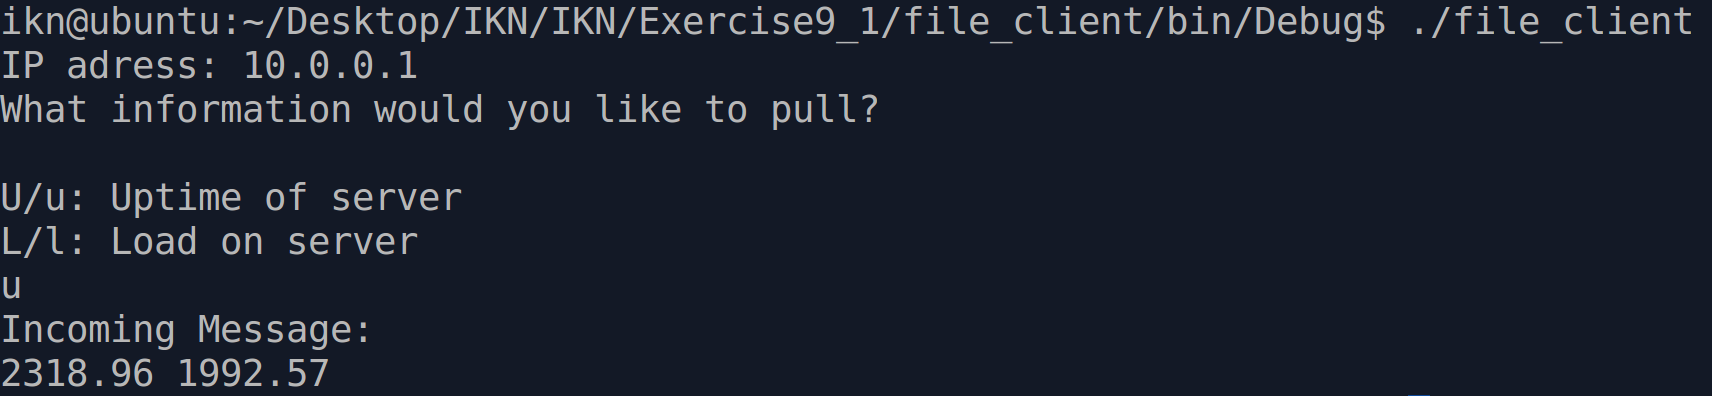
\includegraphics[scale=0.6]{Pic/uptimeclient}}
	\caption{Anmodning om uptime fra klient}
	\label{fig:uptimeclient}
\end{figure} 
\begin{figure}[h!]
	\centering
	\fbox{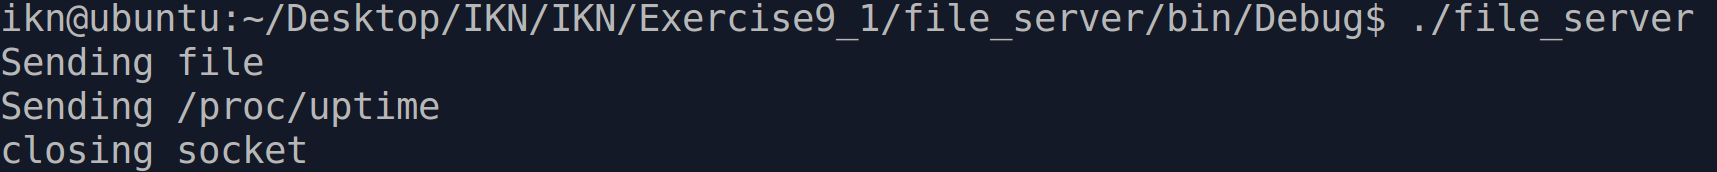
\includegraphics[scale=0.6]{Pic/uptimeserver}}
	\caption{Besvarelse af anmodning om uptime hos server}
	\label{fig:uptimeserver}
\end{figure} 
\begin{figure}[h!]
	\centering
	\fbox{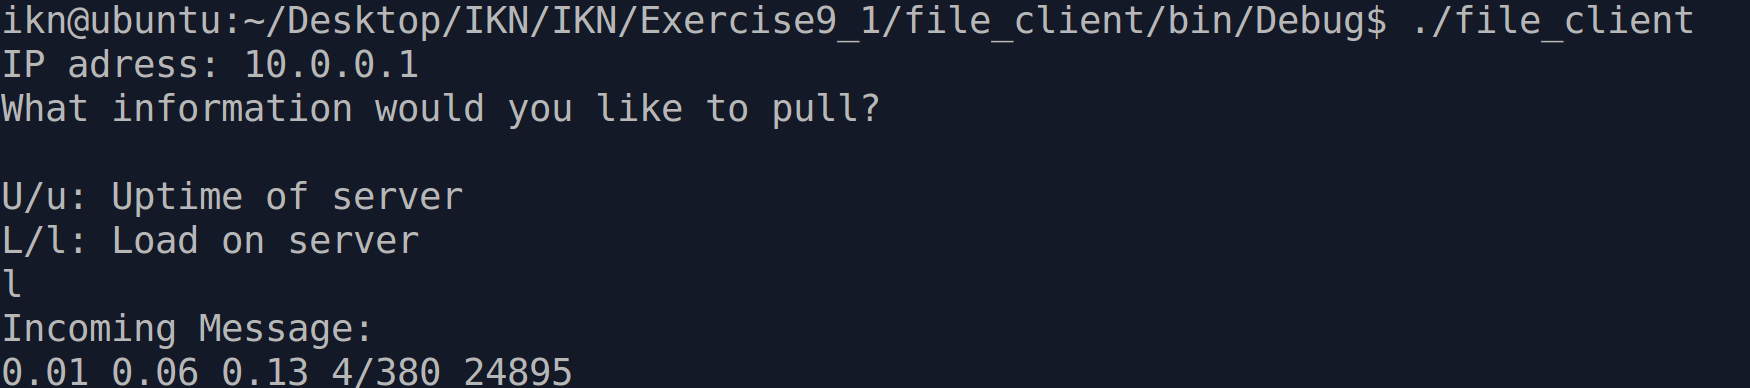
\includegraphics[scale=0.6]{Pic/loadclient}}
	\caption{Anmodning om load fra klient}
	\label{fig:loadclient}
\end{figure} 
\begin{figure}[h!]
	\centering
	\fbox{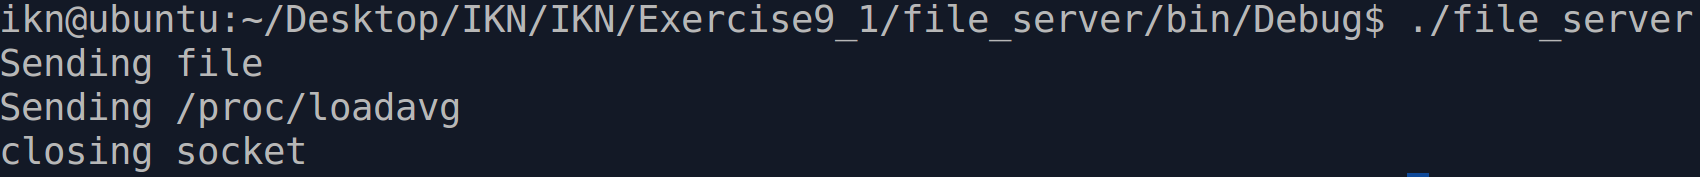
\includegraphics[scale=0.6]{Pic/loadserver}}
	\caption{Besvarelse af anmodning om load hos server}
	\label{fig:loadserver}
\end{figure} 